\addchapheadtotoc
\chapter{Context and related works}

In this chapter, we first introduce graphs and how they arise from real world networks. Then we present the graph classification problem, along with applications in which it arises. Finally, we proceed to detailing state-of-the-art methods and their limitations, before stating our contribution. 
 
\section{Graph structures and its presence in real world}

The need for graphs and their analysis can be traced back to 1679, when G.W.  Leibniz  wrote to C. Huygens about the limitations of traditional analysis methods of geometric figures and said that "we need yet another kind of analysis, geometric or linear, which deals directly with position, as algebra deals with magnitude", \citep{Graph_application}. This lead to graphs, mathematical objects that provide a pictorial and efficient form to represent data with many inter-connections. %With graph structures, these data become easier to be processed and analyzed, and that helps solving many problems that have been unsolved before \citep{Graph_application}.

Formally, a graph of size $v$ is a pair $\mathcal{G}=(\mathcal{V},\mathcal{E})$, where $\mathcal{V}=\{u_1,...,u_v\}$ is a set of $v$ graph nodes (or vertices), and $\mathcal{E}\in \mathcal{V}\times \mathcal{V}$ is the set of edges between these nodes, i.e. $(u_i, u_j)\in \mathcal{E}$ means that the graph has an edge between node $u_i$ and node $u_j$.

Graph structures are used to model a set of objects and their interactions/relations. % that link between different pairs of these objects.  
While the nature of these objects and their interactions vary with the application, the underlying modeling paradigm is the same for all applications: objects are represented by nodes, and a relation between two objects is represented by an edge between the corresponding two nodes. For instance, in a social network like Facebook, nodes are users and edges are friendships between them. In a biological network such as the brain, nodes are brain regions and edges are the nerve connections in between (see Table.\ref{table:Graph_examples} for a list of different examples). 

These graphs, if not too large, can be visually represented in order to provide an intuitive understanding of the existing interactions. Such an illustration is in Fig. \ref{fig:Graph_Example} in the application of chemical reactions.



\begin{figure}[H]
\centering
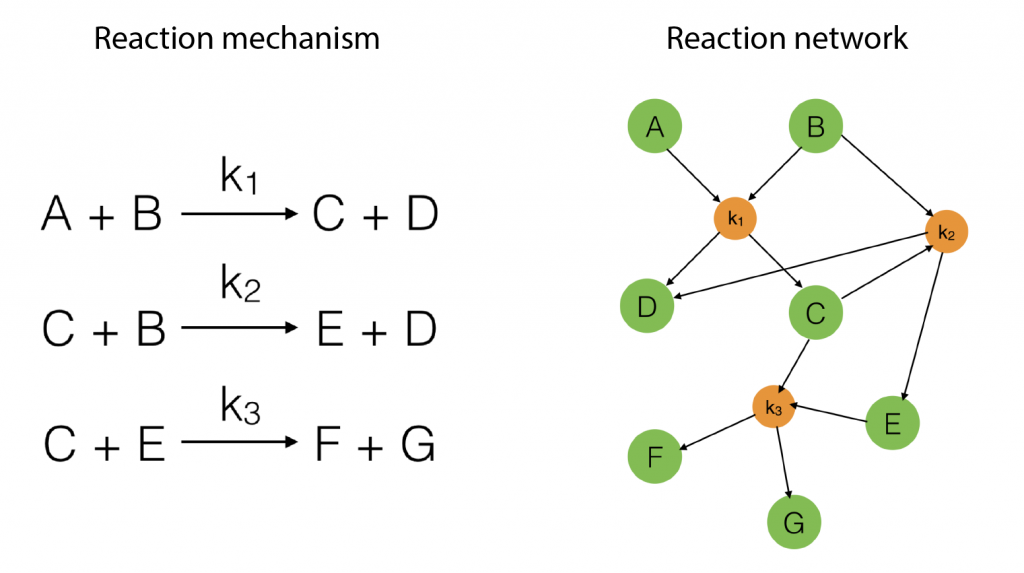
\includegraphics[scale=0.2]{figs/Graph_example.png}
\caption[Graph example to represent Chemical Reactions]{Graph structures in representing chemical reactions mechanisms}
%Source:
\label{fig:Graph_Example}
\end{figure}


\begin{table}
\small
\begin{center}
\begin{tabular}{|c|c|c|c|c|}
\hline
{Network}  &  {Nodes} & {Node features}  & {Edges}  & {Edge features}  \\
\hline
{Transportation system}  &  {cities} & {registered cars}  & {Routes}  & {Length, cost }  \\
\hline
{Banking network}  &  {Account holders} & {account status}  & {Transactions}  & {Transaction value}  \\
\hline
{Social network}  &  {users} & {name, country}  & {Interactions}  & {type (like, comment)}  \\
\hline
\end{tabular}
\end{center}
\caption{Some real world graphs}
\label{table:Graph_examples}
\end{table}

\section{Graph classification problem}
\label{sec:Graph_classification_problem}
Graph classification can be understood in several ways. Here, we place ourselves in the context of \emph{supervised learning}, where we suppose we have access to a set of pre-labeled graphs  $(\mathcal{X}=\{\mathcal{G}_1,\ldots,\mathcal{G}_n\}, \mathcal{Y}=\{y_1,\ldots,y_n\})$, where each graph $\mathcal{G}_i$ is \emph{a priori} known to belong to the class with label $y_i$. Stated simply, the graph classification problem we are interested in in this work may be stated as: given this prior information, design a classification algorithm that, given in input any graph (importantly, any graph belonging or not to $\mathcal{X}$), output the label of the class to which it belongs. 

More formally, consider the set $\mathcal{D}$ of all graphs $\mathcal{G}$ that can occur in some real-world application, a fixed set of classes $\beta=\{\beta _1,\ldots,\beta _l\}$ of finite size $l$, and a mapping function $f:\mathcal{D}\mapsto\beta$ which maps each graph $\mathcal{G}$ in $\mathcal{D}$ to the class $\beta_\mathcal{G}$ it belongs to. Graph classification is the problem of estimating the function $f$ on $\mathcal{D}$ starting from its evaluation on a subset $\mathcal{X}\subset \mathcal{D}$. In other words, we have a dataset $(\mathcal{X}=\{\mathcal{G}_1,\ldots,\mathcal{G}_n\}, \mathcal{Y}=\{y_1,\ldots,y_n\})$ of size $n$ such that $\mathcal{X}\in \mathcal{D}^n$ and $\mathcal{Y}\in\beta^n$, where for each graph $\mathcal{G}_i\in \mathcal{X}$ we have that $y_i=f(\mathcal{G}_i)$ is the class of $\mathcal{G}_i$. The classification task is to have a \textbf{predictive model} which can predict well, based on some-predefined metric,  the class for any new graph $\mathcal{G}$ in $\mathcal{D}$. This prediction functionality of the model is gained using the dataset $(\mathcal{X}, \mathcal{Y})$ to optimize the parameters believed to govern the behavior of $f$ on $\mathcal{D}$. This optimization process is called the learning algorithm.

Note that graph classification as considered here, has nothing to do with the more common problem of \emph{node classification} in a graph. In node classification,  there exists only one graph and the goal is to separate the node set in a partition of communities. In our work, graphs are classified, not nodes. This being said, the extra information that the nodes and/or edges may have in some applications (gender, age for instance for nodes of a social network; maximum bandwidth, number of channels for instance for edges of a communication network; etc.) could in principle be used along with the graph structure to classify different graphs into different classes. However, as the existence of such extra-information is very application-dependent, we prefer to focus here on the case where nodes and edges do not carry such information: the only information one has access to for classification is the graph structure.

Graph classification has been addressed in many different fields of research, such as:
\begin{itemize}
    \item \textbf{\emph{Marketing analytics:}} advertisers and marketers  are interested in detecting the influential people communities in Social Networks in the sense that addressing their products' advertisements to such groups would be a more rewarding investment. This can be approached with graph classification applied on these networks \citep{marketing_analytics}.
    \item \textbf{\emph{Banking security:}} graph classification is used to catch unusual patterns of fraudulent transactions \citep{banking_security}.
    \item \textbf{\emph{Biology and genomics:}} here graphs are based on proteins, such that a nodes correspond
to amino acids that compound the protein.  A pair of amino acids are linked by an edge if they are less than 6 Angstroms apart. The task is to detect whether a protein is an enzyme or not \citep{protein_application}, to mention a few.
\end{itemize}

\section{State-of-the-art methods for graph classification}
\label{section:state}
We  present here existing algorithms for the graph classification problem and discuss their limitations. In general, these algorithms can be classified in four main categories: set based, frequent sub-graph based, kernel based, and graph neural networks based algorithms.\\

\noindent\textbf{Set based algorithms.} This type of algorithms is only applicable to cases where nodes/edges are supplied with features or attributes, as they completely disregard the graph's structure. Based on the provided feature vectors, a distance function of interest between the graphs is computed. % in order to provide a similarity between pairs of edges/nodes in the corresponding sets. 
The drawback of this method is that it does not take the structure (topology) of the graph itself into consideration. For example, if we just compare how much the edges' features of one graph are similar to the edges' features of another, we can have two graphs with arbitrarily different structures but each has the same set of edge features, which will lead to a spurious maximum similarity.
On the other hand, a strength of these algorithms is their low computation cost that is usually linear or quadratic in the number of nodes and edges \citep{graphlet_kernel}.\\
 
\noindent\textbf{Frequent sub-graph based algorithms.} These algorithms contain two steps. First, the graph dataset $\mathcal{X}$ is analyzed to enumerate the frequent sub-graphs occuring in the different graphs. Then, another analysis is done to choose the most discriminative sub-graphs out of the ones found during the first step. The disadvantage of using this method is the computational cost that grows exponentially with the graph size \citep{graphlet_kernel}. \\

\noindent\textbf{Graph kernels based algorithms.} It is a middle ground between both previous methodologies, where the graph structure is well considered, and in most cases, these algorithms are designed in a way that the computational time is a polynomial function of the graph size \citep{graphlet_kernel}. However, some effective and competitive kernels still require exponential time, and this is in short the problem we approach in this work using random features, where our intention is to approximate these kernels or to compete with them in a notably lower computational time. \\

\noindent\textbf{Graph neural networks (GNNs) based algorithms.} GNNs compute a representation vector (embedding vector) for every node in a graph, where this vector is recursively computed by aggregating the representation vectors of neighboring nodes. The goal of this aggregation technique is that nodes that are neighbors (or close) to each other in the graph are more likely to have similar representations (with respect to some similarity function) and vice versa. On the graph level, a representation vector is computed by aggregating its nodes' representation vectors. The result is considered as a usual feature vector of the graph, and it can be fed to a typical deep neural network to learn the classification task. Traditional GNNs such as graph convolutional networks (GCNs) and GraphSAGE perform well when nodes/edges of the graph have feature vectors, but they don't perform well when classifying graphs based only on their topological structure \citep{GCN_powerful}.
However, another GNN structure was developed to overcome this weakness point, and it is referred to by GIN (Graph Isomorphism Network). Regarding the computational time, it is mainly a matter of the layers number in the network, since this parameter in reality represents how far from a node we want to go in order to compute its representation vector. 

\section{Our contribution}
\textbf{Problem:} graphlet kernel is one of the kernel-based algorithms (the third out of the four listed categories), and it has proven to be competitive for graph classification. This kernel takes its input graph, then it enumerates all its sub-graphs of a pre-determined number of nodes (usually small). Next, a function we call later \emph{the matching function} is applied on each of these subgraphs. After that, the average of the results is used to represent the graph. In fact, the number of these sub-graphs drastically increases as the graph becomes larger and contains more nodes. However, the other but the important drawback here is the matching function. Where finding an algorithm to evaluate it in polynomial time of its input dimensionality still an NP problem. 
One way to reduce this computation cost is to consider just a fixed and a reasonable number of sub-graphs instead of the exhaustive enumeration. Still, the matching function is applied on each sub-graph then averaged to represent the main graph. We refer to this method with \emph{graphelt kernel with graph sampling}. As we will see later, this can be seen as enhancement, but it doesn't solve the problem of high computation time.

\textbf{Tools:} random feature maps are randomized functions that map its input to a random element in another space. In addition, each map satisfies the following: if it is applied separately on tow objects,  the inner product of the two results is a random variable, and its expectation is a valid kernel between the input objects. Furthermore, a new technology called \emph{optical processing units (OPUs)} is recently developed, and it has an associate random feature map. The surprise is that this map can be evaluated in light speed.

\textbf{Contribution:} being inspired by graphlet kernel with graph sampling, we:
\begin{enumerate}
    \item Propose a new algorithm, named $GSA-\varphi$, which replaces the matching function in the graphlet kernel with graph sampling technique with any user-defined feature map $\varphi$.
    \item We define the kernel that corresponds to our algorithm, called the mean kernel. Then with concentration inequalities, we prove that our algorithm is concentrated around the mean kernel with high probability. This is with respect to the maximum mean discrepancy (MMD) metric.
    \item After analyzing the OPU structure and its random feature map $\varphi_{OPU}$, We applies our algorithm considering $\varphi_{OPU}$. Our results prove that $GSA-\varphi_{OPU}$ competes the traditional graphlet kernel, and even outperform its approximation with graph sampling. Of course, this is with $O(1)$ in input dimensionality.
    \item We use Gaussian random feature map in our algorithm, and it also competes graphlet kernel.
    \item We benchmark our algorithm against graph convolution networks, and results show that our algorithm with $\varphi_{OPU}$ performs better.
\end{enumerate}

Without promising results, we tried also to apply Eigenvalue decomposition on each sub-graph before passing it to our algorithm. We did that to have equivalent behavior to the matching function, but results proved that to be not true.

